%noindent
Este anexo resume cotizaciones referenciales asociadas a la fabricación de las \ac{PCB}s del prototipo, así como opciones de envío y servicios adicionales disponibles en plataformas de compra y manufactura.

\section{Cotización de manufactura y servicios de \ac{PCB} mediante JLCPCB}

Se cotizaron dos \ac{PCB}s de dos capas: una para control y registro de datos, y otra para el sensado con un sensor de efecto \textit{Hall}. La estimación se realizó con la herramienta de cotización en línea de JLCPCB, la cual incluye costos de manufactura, envío internacional y servicios como ensamble y plantilla de soldadura \textit{stencil} \cite{jlcpcb_quote_es}.

De acuerdo con la cotización realizada, el costo de manufactura resulta reducido en comparación con el costo de envío internacional, el cual depende del método de transporte y del peso del paquete.

El servicio de ensamble permite reducir el esfuerzo de adquisición de componentes importados, ya que la plataforma integra el abastecimiento y el montaje. En este caso, el costo total y el envío tienden a incrementarse debido al mayor peso. Además, el ensamble puede solicitarse en cantidades menores, lo cual es consistente con el enfoque de prototipado del banco de pruebas en un nivel de madurez TRL 4 indicado en el Capítulo \ref{ch:CH01}.

Una alternativa intermedia consiste en solicitar solo la manufactura e incluir una plantilla de soldadura \textit{stencil} para facilitar el soldado rápido de componentes adquiridos localmente. Esta opción suele ser menor que el ensamble en cuanto a costo se refiere; sin embargo, la plantilla representa un costo adicional relevante.

\begin{table}[H]
\centering
\caption{Resumen comparativo de costos para tres alternativas de adquisición.}
\label{tab:jlcpcb_resumen_costos}
\begin{tabular}{|l|c|c|c|}
\hline
\multicolumn{1}{|c|}{Manufactura y otros servicios} & Costo por servicios & Costo de envío & Costo total \\
\hline
Solo manufactura de dos \ac{PCB}s & US\$ 10.80 & US\$ 34.56 & US\$ 45.36 \\
\hline
Manufactura con ensamble & US\$ 132.99 & US\$ 49.00 & US\$ 172.99 \\
\hline
Manufactura con plantilla \textit{stencil} & US\$ 24.80 & US\$ 63.46 & US\$ 88.26 \\
\hline
\end{tabular}
\caption*{\textit{Nota: Fecha de consulta: miércoles 04 de febrero de 2026.}}
\end{table}


\section{Cotización de componentes electrónicos}

A continuación, se presenta la cotización de componentes que no se encontraron en el mercado local, por lo que se consideran precios de importación. En este caso, se tomó como referencia Mouser Perú, debido a que facilita la adquisición de componentes desde el exterior con entrega al país. \autocite{mouser_pe_componentes}

\begin{table}[H]
\centering
\caption{Costo referencial de componentes electrónicos importados.}
\label{tab:4.Costo_componentes_mouser}
\begin{tabular}{|l|c|c|c|}
\hline
\multicolumn{1}{|c|}{Ítem} & Proveedor & Cant. & Precio S/. \\
\hline
Diodo TVS SM4T28CAY & Mouser Perú & 1 & 3.27 \\
\hline
Regulador LM2594M-3.3/NOPB & Mouser Perú & 1 & 18.22 \\
\hline
Driver VNH7070BASTR & Mouser Perú & 1 & 13.23 \\
\hline
Sensor TMAG5170A1QDGKR & Mouser Perú & 1 & 11.37 \\
\hline
\multicolumn{3}{|c|}{Costo total} & 46.09 \\
\hline
\end{tabular}
\caption*{\textit{Nota: Fecha de consulta: miércoles 04 de febrero de 2026.}}
\end{table}

Además del costo de los componentes, el pedido considera cargos por envío y, cuando aplique, costos de importación como aranceles, aduana e impuestos. \autocite{mouser_envio_tarifa_plana}. Para esta cotización, el costo de envío mostrado en la plataforma corresponde a S/ 200.00. La selección del método de envío se define principalmente por el plazo de entrega y las condiciones de cobro al destinatario.

\begin{table}[H]
\centering
\caption{Lista de costos de los componentes electrónicos}
\label{tab:costos_electronicos_anexo}

\begin{tblr}[
  theme = pucp,
]{
  width=\linewidth,
  colspec = {
    X[3.2,l,m]
    X[0.7,c,m]
    X[0.9,c,m]
    X[1.1,c,m]
    X[1.1,c,m]
    X[1.0,c,m]
  },
  colsep=2pt,
  rowsep=1pt,
  rows={font=\footnotesize},
  row{1}={font=\footnotesize\bfseries,halign=c,valign=m},
  row{Z}={font=\footnotesize\bfseries},
  hlines, vlines,
}
Componente
  & Cant.
  & Prov.
  & \shortstack[c]{Precio\\unit.\\(S/.)}
  & \shortstack[c]{Precio\\total\\(S/.)}
  & \shortstack[c]{Precio\\total\\(US\$)} \\

Pulsador \SI{6}{mm}$\times$\SI{6}{mm} (2 pines)
  & 2 & Prov-A & 0.30 & 0.60 & 0.18 \\
Condensador SMD 1206 (\SI{2.2}{nF})
  & 1 & Prov-B & 0.50 & 0.50 & 0.15 \\
Condensador SMD 1206 (\SI{10}{nF})
  & 1 & Prov-B & 0.50 & 0.50 & 0.15 \\
Condensador SMD 1206 (\SI{100}{nF})
  & 5 & Prov-B & 0.50 & 2.50 & 0.74 \\
Condensador SMD 1206 (\SI{1}{\micro\farad})
  & 2 & Prov-B & 0.50 & 1.00 & 0.30 \\
Condensador electrolítico SMD (\SI{1}{\micro\farad})
  & 1 & Prov-B & 1.00 & 1.00 & 0.30 \\
Condensador electrolítico SMD (\SI{330}{\micro\farad})
  & 1 & Prov-B & 0.80 & 0.80 & 0.24 \\
Condensador electrolítico SMD (\SI{470}{\micro\farad})
  & 1 & Prov-B & 0.50 & 0.50 & 0.15 \\
Diodo Schottky SS36
  & 2 & Prov-A & 0.30 & 0.60 & 0.18 \\
SM4T28CAY
  & 1 & Prov-C & 3.27 & 3.27 & 0.97 \\
Fusible
  & 1 & Prov-A & 1.00 & 1.00 & 0.30 \\
Porta fusible
  & 1 & Prov-A & 0.80 & 0.80 & 0.24 \\
Conector JST (2 pines)
  & 3 & Prov-A & 0.60 & 1.80 & 0.53 \\
Header macho de 40 pines
  & 1 & Prov-A & 3.90 & 3.90 & 1.16 \\
Bobina \SI{47}{\micro H} SMD (\SI{12.3}{mm}$\times$\SI{12.3}{mm})
  & 1 & Prov-B & 2.80 & 2.80 & 0.83 \\
LED SMD 1206 (rojo)
  & 2 & Prov-B & 0.30 & 0.60 & 0.18 \\
Bornera
  & 1 & Prov-A & 0.70 & 0.70 & 0.21 \\
Transistor NPN \SI{25}{V} \SI{300}{mA} (SOT-23)
  & 2 & Prov-B & 0.20 & 0.40 & 0.12 \\
Resistencia SMD 1206 (\SI{47}{k\ohm})
  & 2 & Prov-B & 0.20 & 0.40 & 0.12 \\
Resistencia SMD 1206 (\SI{10}{k\ohm})
  & 9 & Prov-B & 0.20 & 1.80 & 0.53 \\
Resistencia SMD 1206 (\SI{1}{k\ohm})
  & 3 & Prov-B & 0.20 & 0.60 & 0.18 \\
Resistencia SMD 1206 (\SI{100}{\ohm})
  & 2 & Prov-B & 0.20 & 0.40 & 0.12 \\
Resistencia SMD 1206 (\SI{470}{\ohm})
  & 2 & Prov-B & 0.20 & 0.40 & 0.12 \\
Resistencia SMD 1206 (\SI{4.7}{k\ohm})
  & 1 & Prov-B & 0.20 & 0.20 & 0.06 \\
Resistencia SMD 1206 (\SI{5.1}{k\ohm})
  & 2 & Prov-B & 0.20 & 0.40 & 0.12 \\
VNH7070BASTR
  & 1 & Prov-C & 0.20 & 0.20 & 0.06 \\
LM2594M-3.3
  & 1 & Prov-C & 18.22 & 18.22 & 5.41 \\
ESP32-WROOM-32D-N4
  & 1 & Prov-B & 17.00 & 17.00 & 5.04 \\
Módulo ENC28J60
  & 1 & Prov-B & 22.00 & 22.00 & 6.53 \\
USB-TYPE-C-018
  & 1 & Prov-A & 0.70 & 0.70 & 0.21 \\
TMAG5170A1QDGKT
  & 1 & Prov-C & 11.37 & 11.37 & 3.37 \\
\SetCell[c=4]{r}{\bfseries Total} & 96.96 & 28.77 \\
\end{tblr}
\end{table}

\begin{flushleft}
\footnotesize\textit{Nota:} Prov-A = Hi-Fi Electrónica; Prov-B = Stacktronics; Prov-C = Mouser.
\end{flushleft}

\begin{table}[H]
\centering
\caption{Costo referencial de \ac{PCB}s fabricadas para pruebas}
\label{tab:costo_pcbs_pruebas}
\begin{tabular}{|l|c|c|c|}
\hline
\multicolumn{1}{|c|}{Ítem} & Proveedor & Cant. & Precio S/. \\
\hline
\ac{PCB} de pruebas TMAG5170 & Mercado peruano & 1 & 20 \\
\hline
\ac{PCB} de pruebas VNH7070BAS & Mercado peruano & 1 & 20 \\
\hline
\multicolumn{3}{|c|}{Costo total} & 40 \\
\hline
\end{tabular}
\end{table}

% %noindent
% Este anexo resume cotizaciones referenciales asociadas a la fabricación de las \ac{PCB}s del prototipo, así como opciones de envío y servicios adicionales disponibles en plataformas de compra y manufactura.

% \section{Cotización de manufactura y servicios de \ac{PCB} mediante JLCPCB}
% Se cotizaron dos \ac{PCB}s de dos capas: una para control y registro de datos, y otra para el sensado con un sensor de efecto \textit{Hall}. La estimación se realizó con la herramienta de cotización en línea de JLCPCB, la cual incluye costos de manufactura, envío internacional y servicios como ensamble y plantilla de soldadura \textit{stencil} \cite{jlcpcb_quote_es,jlcpcb_pcba}.

% \begin{figure}[H]
%     \centering
%     \begin{subfigure}[t]{0.49\linewidth}
%         \centering
%         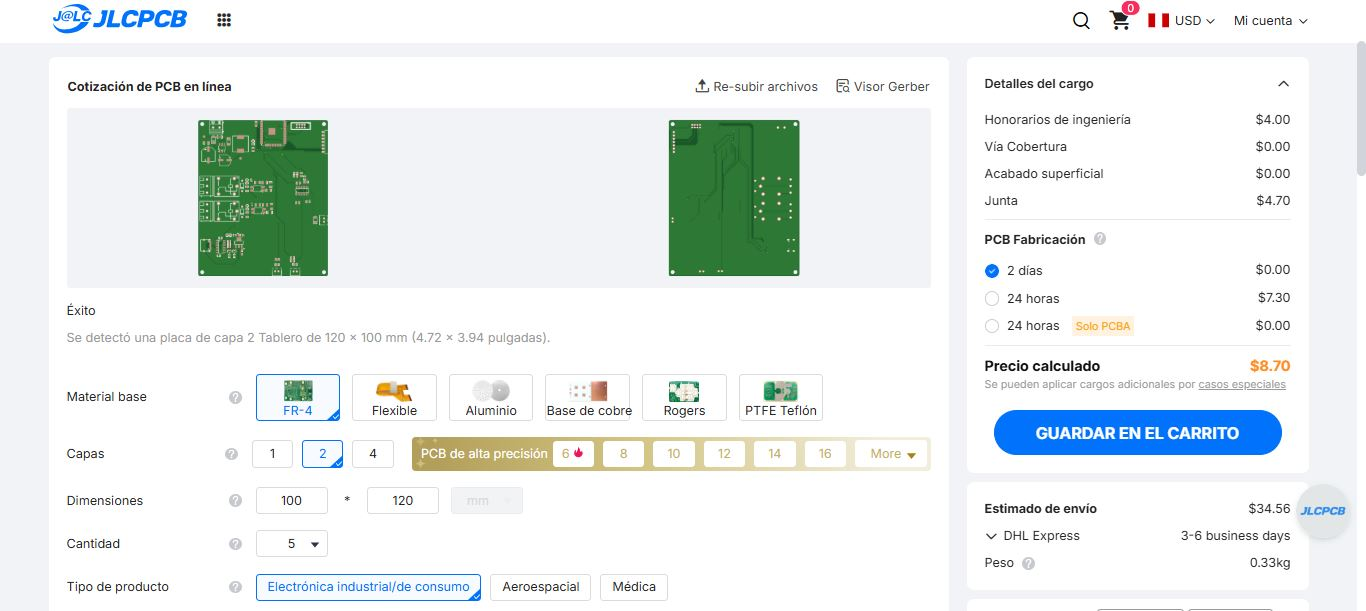
\includegraphics[width=\linewidth]{ANNEX/Fig/AZ/cotizacion_JLCSC_CNTRL.JPG}
%         \caption{Cotización de la \ac{PCB} de control y registro de datos.}
%         \label{fig:jlcpcb_quote_control}
%     \end{subfigure}\hfill
%     \begin{subfigure}[t]{0.49\linewidth}
%         \centering
%         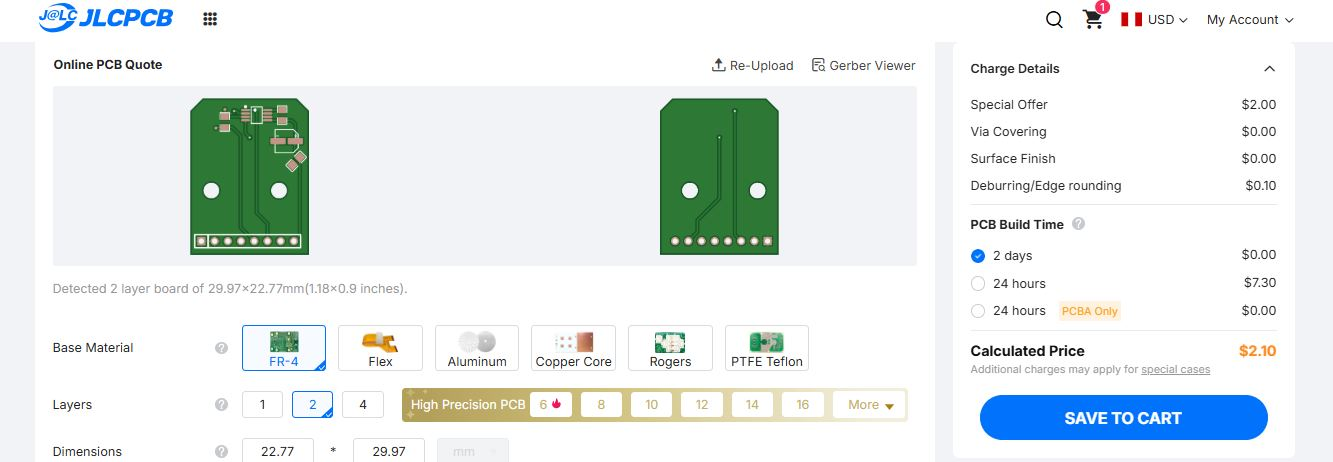
\includegraphics[width=\linewidth]{ANNEX/Fig/AZ/cotizacion_JLCSC_SENSOR.JPG}
%         \caption{Cotización de la \ac{PCB} del sensor de efecto \textit{Hall}.}
%         \label{fig:jlcpcb_quote_sensor}
%     \end{subfigure}
%     \caption{Cotizaciones individuales de manufactura obtenidas desde la plataforma de JLCPCB.}
%     \label{fig:jlcpcb_quote_pcbs}
% \end{figure}

% De acuerdo con la Figura \ref{fig:jlcpcb_quote_pcbs}, el costo de manufactura es reducido frente al costo de envío internacional, el cual depende del método de transporte y del peso del paquete. Las alternativas de envío disponibles se muestran en la Figura \ref{fig:jlcpcb_shipping_pcb}.

% \begin{figure}[H]
%     \centering
%     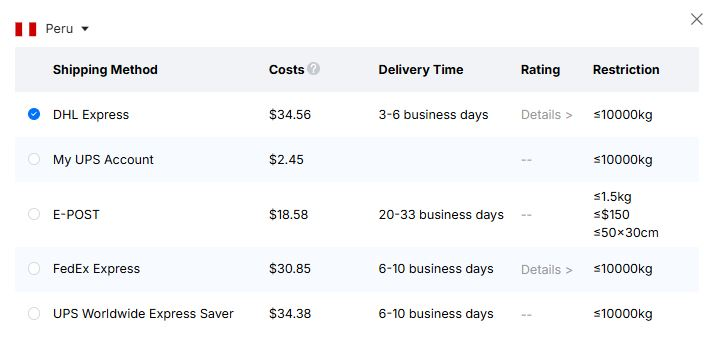
\includegraphics[width=0.92\linewidth]{ANNEX/Fig/AZ/SHIPPING_METHOD.JPG}
%     \caption{Opciones de envío internacional mostradas por JLCPCB para la manufactura de \ac{PCB}.}
%     \label{fig:jlcpcb_shipping_pcb}
% \end{figure}

% % Si cuentas con una captura del carrito con solo manufactura de ambas \ac{PCB}s y envío,
% % insértala aquí y actualiza el nombre del archivo.
% % \begin{figure}[!t]
% %     \centering
% %     \includegraphics[width=0.92\linewidth]{ANNEX/Fig/AZ/Carrito_JLCPCB_Manuf.JPG}
% %     \caption{Costo total referencial en carrito para manufactura de ambas \ac{PCB}s y envío internacional.}
% %     \label{fig:jlcpcb_cart_manuf}
% % \end{figure}

% El servicio de ensamble permite reducir el esfuerzo de adquisición de componentes importados, ya que la plataforma integra el abastecimiento y el montaje. En este caso, el costo total y el envío tienden a incrementarse debido al mayor peso, tal como se aprecia en la Figura \ref{fig:jlcpcb_cart_assembly} y en la Figura \ref{fig:jlcpcb_shipping_assembly}. Además, el ensamble puede solicitarse en cantidades menores, lo cual es consistente con el enfoque de prototipado del banco de pruebas en un nivel de madurez TRL 4 indicado en el Capítulo \ref{ch:CH01}.

% \begin{figure}[H]
%     \centering
%     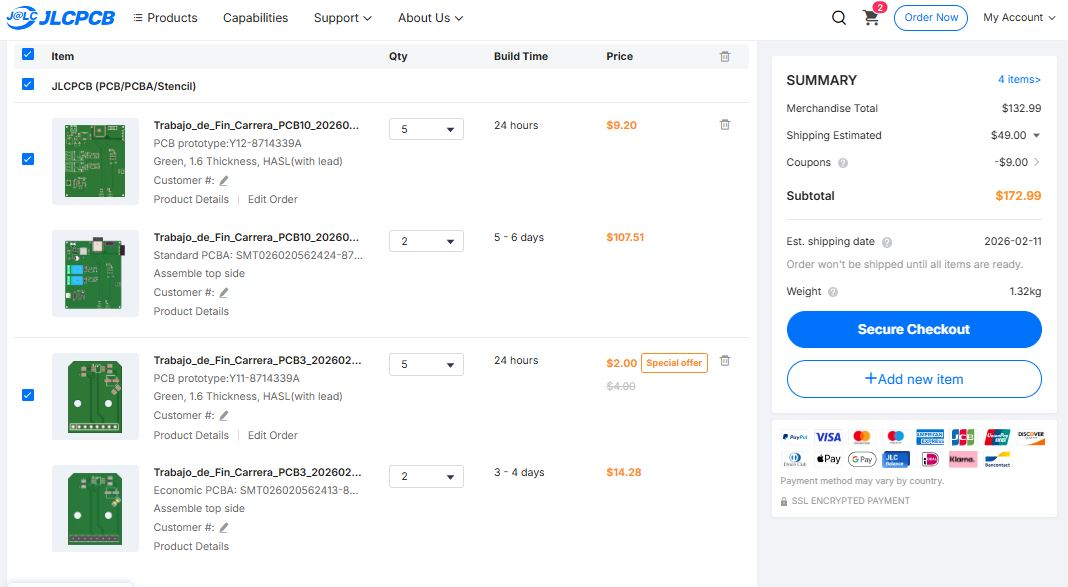
\includegraphics[width=0.92\linewidth]{ANNEX/Fig/AZ/Carrito_JLCSC_Asem.JPG}
%     \caption{Cotización en carrito considerando ensamble y envío internacional.}
%     \label{fig:jlcpcb_cart_assembly}
% \end{figure}

% \begin{figure}[H]
%     \centering
%     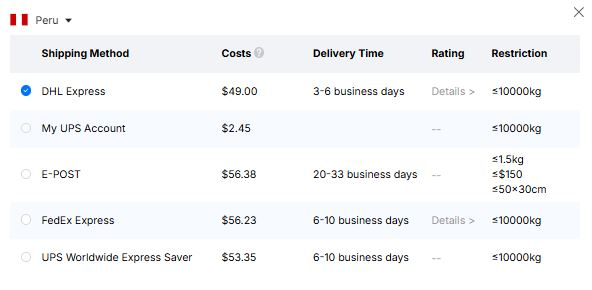
\includegraphics[width=0.92\linewidth]{ANNEX/Fig/AZ/SHIPPING_METHOD_asse.JPG}
%     \caption{Opciones de envío internacional mostradas por JLCPCB para la cotización con ensamble.}
%     \label{fig:jlcpcb_shipping_assembly}
% \end{figure}

% Una alternativa intermedia consiste en solicitar solo la manufactura e incluir una plantilla de soldadura \textit{stencil} para facilitar el soldado rápido de componentes adquiridos localmente. Esta opción suele ser menor que el ensamble en cuanto a costo s refiere, aunque, de igual forma la paantilla representa un costo adicional relevante, como se observa en la Figura \ref{fig:jlcpcb_cart_stencil}.

% \begin{figure}[H]
%     \centering
%     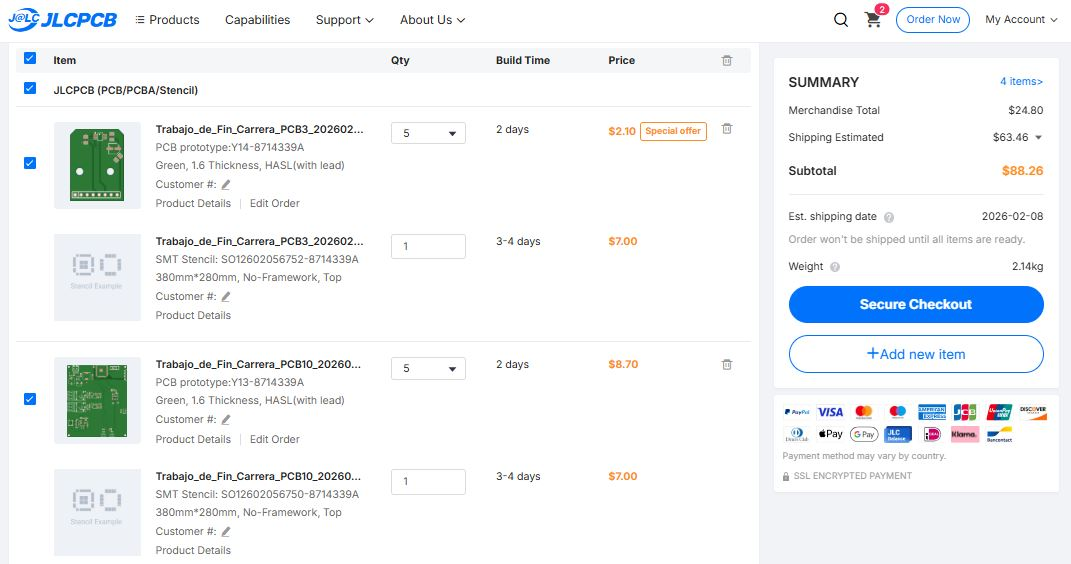
\includegraphics[width=0.92\linewidth]{ANNEX/Fig/AZ/Carrito_JLCSC_stensil.JPG}
%     \caption{Cotización en carrito considerando manufactura de \ac{PCB} y plantilla de soldadura \textit{stencil}.}
%     \label{fig:jlcpcb_cart_stencil}
% \end{figure}

% % Si tienes una captura específica de envío para el caso con plantilla, reemplaza el archivo.
% \begin{figure}[H]
%     \centering
%     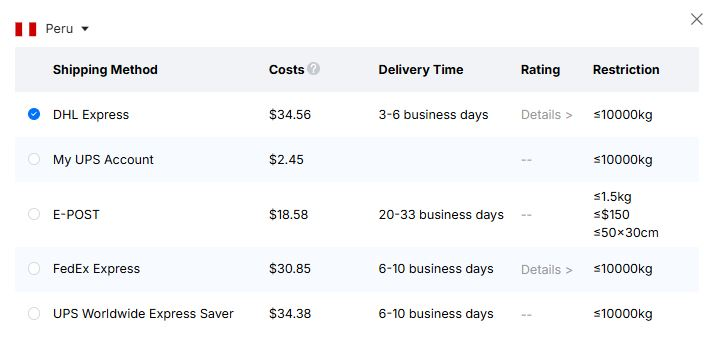
\includegraphics[width=0.92\linewidth]{ANNEX/Fig/AZ/SHIPPING_METHOD.JPG}
%     \caption{Opciones de envío internacional para el caso con plantilla de soldadura \textit{stencil}.}
%     \label{fig:jlcpcb_shipping_stencil}
% \end{figure}

% \begin{table}[H]
% \centering
% \caption{Resumen comparativo de costos para tres alternativas de adquisición.}
% \label{tab:jlcpcb_resumen_costos}
% \begin{tabular}{|l|c|c|c|}
% \hline
% \multicolumn{1}{|c|}{Manufactura y otros servicios} & Costo por servicios & Costo de envío & Costo total \\
% \hline
% Solo manufactura de dos \ac{PCB}s & US\$ 10.80 & US\$ 34.56 & US\$ 45.36 \\
% \hline
% Manufactura con ensamble & US\$ 132.99 & US\$ 49.00 & US\$ 172.99 \\
% \hline
% Manufactura con plantilla \textit{stencil} & US\$ 24.80 & US\$ 63.46 & US\$ 88.26 \\
% \hline
% \end{tabular}
% \caption*{\textit{Nota: Fecha de consulta: miércoles 04 de febrero de 2026.}}
% \end{table}



% \section{Cotización de componentes electrónicos}
% A continuación, se presenta la cotización de componentes que no se encontraron en el mercado local, por lo que se consideran precios de importación. En este caso, se tomó como referencia Mouser Perú, debido a que facilita la adquisición de componentes desde el exterior con entrega al país. \autocite{mouser_pe_componentes}


% En la Figura \ref{fig:cotizacion_mouser_capturas} se muestran las capturas de la cotización referencial para cada componente.

% \begin{figure}[H]
% \centering
% \begin{subfigure}[t]{0.48\textwidth}
%   \centering
%   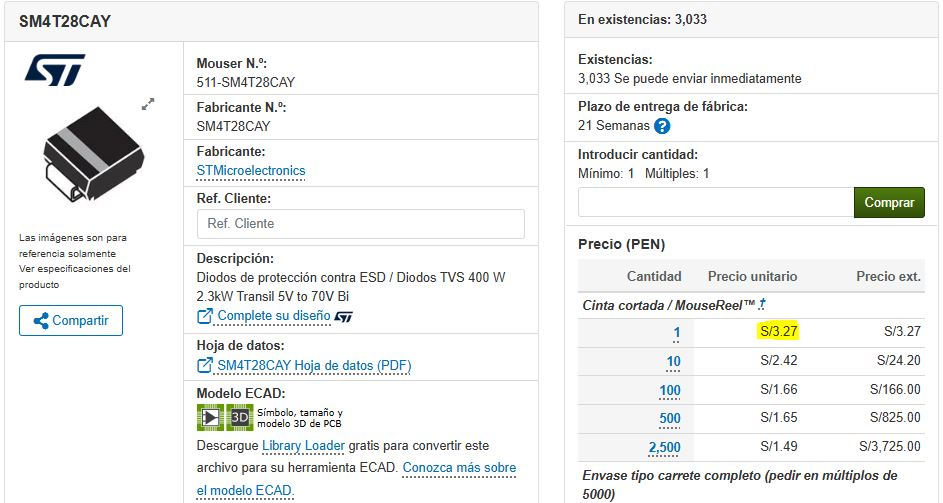
\includegraphics[width=\linewidth]{ANNEX/Fig/AZ/diodo_mouser.JPG}
%   \caption{Diodo TVS SM4T28CAY. \autocite{mouser_sm4t28cay}}
%   \label{fig:mouser_sm4t28cay}
% \end{subfigure}
% \hfill
% \begin{subfigure}[t]{0.48\textwidth}
%   \centering
%   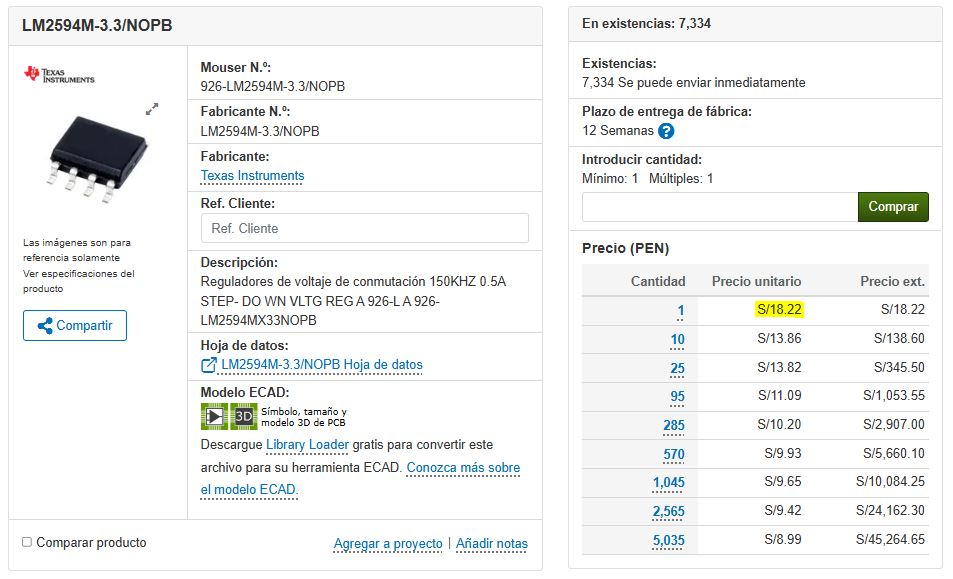
\includegraphics[width=\linewidth]{ANNEX/Fig/AZ/reg_mouser.JPG}
%   \caption{Regulador LM2594M-3.3/NOPB. \autocite{mouser_lm2594m33}}
%   \label{fig:mouser_lm2594m33}
% \end{subfigure}

% \vspace{0.6em}

% \begin{subfigure}[t]{0.48\textwidth}
%   \centering
%   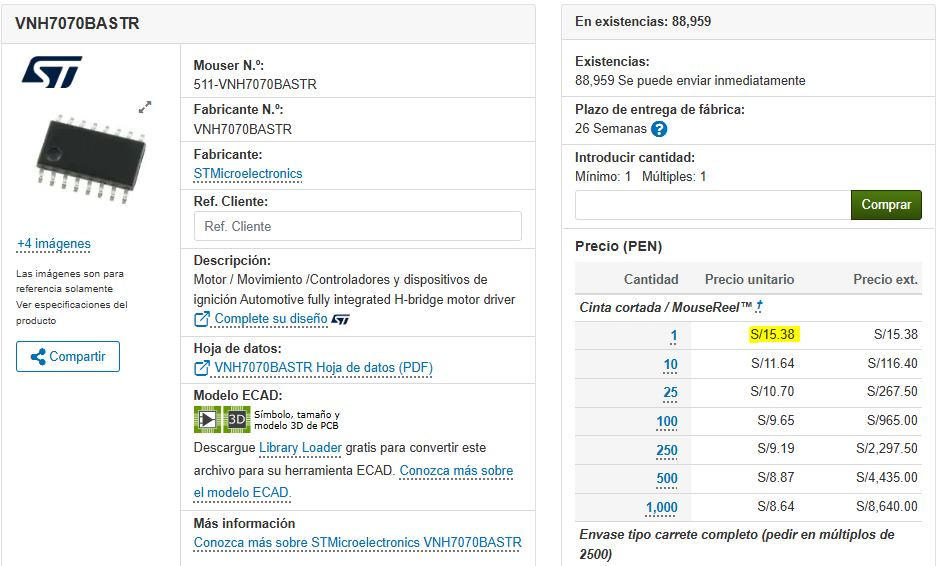
\includegraphics[width=\linewidth]{ANNEX/Fig/AZ/driver_mouser.JPG}
%   \caption{Driver VNH7070BASTR. \autocite{mouser_vnh7070bastr}}
%   \label{fig:mouser_vnh7070}
% \end{subfigure}
% \hfill
% \begin{subfigure}[t]{0.48\textwidth}
%   \centering
%   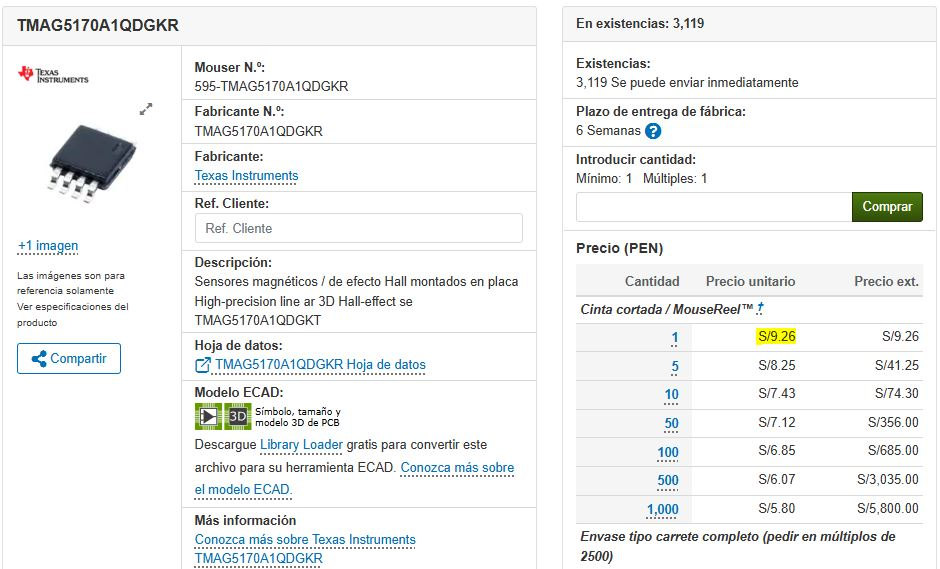
\includegraphics[width=\linewidth]{ANNEX/Fig/AZ/TMAG5170_mouser.JPG}
%   \caption{Sensor TMAG5170A1QDGKR. \autocite{mouser_tmag5170}}
%   \label{fig:mouser_tmag5170}
% \end{subfigure}

% \caption{Capturas de la cotización referencial en Mouser Perú para componentes importados.}
% \label{fig:cotizacion_mouser_capturas}
% \end{figure}

% \begin{table}[H]
% \centering
% \caption{Costo referencial de componentes electrónicos importados.}
% \label{tab:4.Costo_componentes_mouser}
% \begin{tabular}{|l|c|c|c|}
% \hline
% \multicolumn{1}{|c|}{Ítem} & Proveedor & Cant. & Precio S/. \\
% \hline
% Diodo TVS \texttt{SM4T28CAY}            & Mouser Perú & 1 & 3.27 \\
% \hline
% Regulador \texttt{LM2594M-3.3/NOPB}     & Mouser Perú & 1 & 18.22 \\
% \hline
% Driver \texttt{VNH7070BASTR}           & Mouser Perú & 1 & 13.23 \\
% \hline
% Sensor \texttt{TMAG5170A1QDGKR}         & Mouser Perú & 1 & 11.37 \\
% \hline
% \multicolumn{3}{|c|}{Costo total} & 46.09 \\
% \hline
% \end{tabular}
% \caption*{\textit{Nota: Fecha de consulta: miércoles 04 de febrero de 2026.}}
% \end{table}




% Además del costo de los componentes, el pedido considera cargos por envío y, cuando aplique, costos de importación como aranceles, aduana e impuestos. \autocite{mouser_envio_tarifa_plana}
% Para esta cotización, el costo de envío mostrado en la plataforma corresponde a S/ 200.00.

% En la Figura \ref{fig:mouser_opciones_envio} se muestran alternativas de envío disponibles al momento de la consulta. En este caso, el costo se mantiene prácticamente constante entre opciones, por lo que la selección se define principalmente por el plazo de entrega y las condiciones de cobro al destinatario.

% \begin{figure}[H]
%   \centering
%   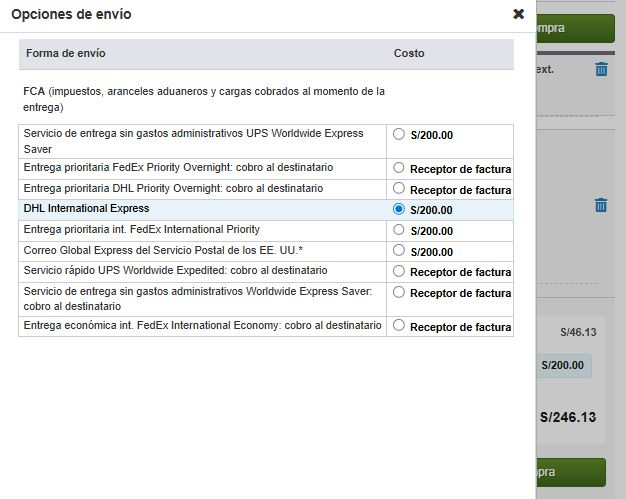
\includegraphics[width=0.82\linewidth]{ANNEX/Fig/AZ/opciones_envio.JPG}
%   \caption{Opciones de envío mostradas por Mouser Perú para la cotización consultada.}
%   \label{fig:mouser_opciones_envio}
% \end{figure}
